\chapter{Grundlagen}
    \section{Einkristalloberflächen}
        \begin{itemize}
            \item Oberflächen aus FK
            \item Rekonstruktion
            \item Elektronische Struktur (Oberflächenzustände)
            \item Antiferromagneten
        \end{itemize}

    \section{Antiferromagneten}
        Antiferromagneten (AFM) seichen sich dadurch aus, dass Sie nach außen hin kein permanetes magnetisches Moment aufweisen.
        Vereinfacht sind im Inneren die magnetischen Momente vom gleichen Betrag und nebeneinander liegende Momente sind antiparallel unterinander ausgerichtet.
        Dieser Zustand ist allerdings nur unterhalb der Néel-Temperatur stabil, oberhalb verhält sich die AFM paramagnetisch.
    
    \section{WW von Oberfläche mit Molekülen}
        \cite{ma-DJ}
        \begin{itemize}
            \item Selbstanordnung
            \item Energie level anpassung
        \end{itemize}
        Bei der Wechselwirkung (WW) von Molekülen mit Oberflächen wird in zwei Arten der Adsorption unterschieden. 
        Zum Einen der Physisorption und der Chemisorption, welche wiederum in stark und schwach unterschieden wird.
        Zwischen den beiden Adsorptionsarten lässt sich durch ihre Bindungsstärke von den Molekülen auf dem Substrat unterscheiden.

        \subsection{Physisorption}
            Bei der Physisorption spielt maßgeblich die Van-der-Waals-Kraft eine Rolle, hat also eine eher eine geringer Bindungsenergie der Moleküle zum Substrat.
            Die Van-der-Waals-Kraft gehört zu den elektrostatischen Kräften, es werden also keine Elektronen mit dem Substrat ausgetauscht.
            Allein die induzierung und fluktuation von Dipolen führt zu dieser Bindung zwischen Molekül und Substrat.
            Da die Wechselwirkung bei der Physisorption nur gering ist werden die Eigenschaften der Oberfläche und des Moleküles nur schwach beeinflusst.
            Beim Substrat kann es zu Relaxation kommen.
            Die Bindungen des Moleküls werden nur schwach beeinflusst, sodass sie den Eigenschaften aus der Gasphase stark ähneln.
            Bei den Van-der-Waals-Kräften kann man in drei Arten uterteilen:
            \begin{itemize}
                \item \textbf{Dipol-Dipol-Kraft:} Sie ist die Kraft zwischen zwei Dipolen, die Keeson-Wechselwirkung.
                \item \textbf{Dipol-induzierter-Dipol-Kraft:} Die Wechselwirkung zwischen einem induziertem Dipol und einem Dipol wird auch als Debye-Wechselwirkung bezeichnet.
                \item \textbf{Londonsche Dispersions-Wechselwirkung:} Zwischen zwei induzierten Dipolen wirkt die Londonsche Dispersions-Wechselwirkung, sie dominiert meist die 
            \end{itemize}
        
        
        \subsection{Chemisorption}
            Im Gegensatz zur Physisorption findet bei der Chemisorption meist ein austausch von Elektronen statt, der chemischen Bindung.
            Diese Bindungen sind um Einiges stärker als die der Physisorption und führen somit zu Veränderung am Substrat wie auch den Molekülen.
            \textbf{Chemisorption nicht nur von der stärke der WW zu unterscheiden, auch, dass chemische Veränderung auftritt.
            Abstand Molekül/Substrat eine Rolle?}
            NiO zeigt für einige Moleküle Chemisorption, was durch enthaltene Defekt hervorgerufen wird \cite{kunz_chemisorption_1985}.
            
    \section{Gold (111) Oberfläche}
        \textbf{\cite{5A_1}}
        Ebenenabstand in Au(111) $d_0 = \SI{2.35}{\angstrom}$.

        \begin{itemize}
            \item Rekonstruktion
            \item WKF
            \item fcc Struktur, Gitterkonstante  $a=\SI{4.08}{\angstrom}$ \cite{Marx}.
            \item Gold (Au) is a noble metal. Its conductivity, stability and the fact that it is not reacting much with the adsorbate, make it a common substrate for the PES measurement in UHV conditions.
        \end{itemize}


    \section{Nickeloxid (111) Oberfläche}
        \begin{itemize}
            \item AFM
            \item Charge-Transferisolator (vergleich Mott-Hubbard)
            \item WKF
            \item Rekonstruktionen
            \item Gitterparameter
            \item NaCl Struktur
        \end{itemize}
        NiO ist eine Antiferromagnet mit einer Neél-Temperatur von \SI{525}{\kelvin} \cite{kunz_chemisorption_1985}.
        Mit der Gitterstruktur von \ce{NaCl} \cite{kunz_chemisorption_1985}.
        Das 3d Ni Band ist nur teilgefüllt mit acht von zehn möglichen Elektronen und doch ein Isolator \cite{kunz_chemisorption_1985}.
        Die thermische Bandlücke liegt bei \SI{3.6}{\electronvolt} \cite{kunz_chemisorption_1985}.

        Warum NiO - weil AFM -> Spinwellen, und Isolator keine Elektronen bewegung keine Joulsche Wärme

        AFM und Moleküle? -> Interface: Molekül anregen -> durch Kopplung SW in AFM auslösen -> anderes Molekül nimmt Spinwelle auf (THz, also sehr schnell)

    \section{Pentacene/PEN/5A}
        \begin{itemize}
            \item Geometrische Struktur
            \item Orbital Struktur
        \end{itemize}
        Pentacene oder auch PEN, 5A genannt hat eine Dichte von \SI{1.232(6)}{\gram\per\cubic\centi\meter} \cite{CAS}.
        \ce{C22H14}
        \begin{figure}
            \centering
            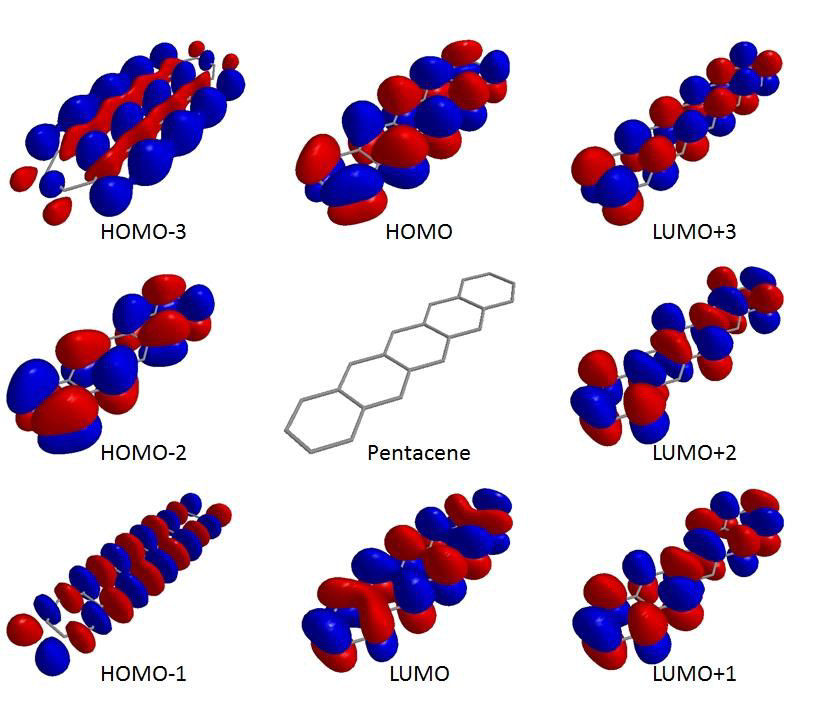
\includegraphics[width=0.3\textwidth]{./content/PEN.jpg}
            \caption{Geometrische Struktur des Pentacene sowei die vier höchsten besetzten und vier niedrigesten unbesetzen Orbitale. Vorlage aus \cite{PEN}.}
            \label{fig:PEN}
        \end{figure}
        
        \textbf{\cite{5A_1}}
        Pentacene ist ein Elektronendonator (gibt gerne Elektronen ab) und zeigt Physisorption auf Au(111).
        Ist ein p-Typ Halbleiter
        Pentacene hat eine hohe Elktronenbeweglichkeit in dünnen Filmen
        PEN auf Au(111) zeigt einen Substrat Molekülabstand von \SI{3.28}{\angstrom} - typisch für Physisorption
        PEN liegt glatt auf Au(111)
    